\documentclass[11pt]{article}

\usepackage{fancyhdr}
\pagestyle{fancy}
\fancyhf{} % clear default header/footer
\fancyhead[C]{Working Notes: Claims Not Verified --- companion to theory\_to\_algorithm\_joery.tex}
\renewcommand{\headrulewidth}{0.4pt}

\usepackage[margin=1in]{geometry}
\usepackage[T1]{fontenc}
\usepackage[utf8]{inputenc}
\usepackage{amsmath,amssymb,amsthm,mathtools}
\usepackage{tikz}
\usetikzlibrary{positioning}
\usepackage{booktabs}
\usepackage{enumitem}
\usepackage{xcolor}
\usepackage[colorlinks=true,linkcolor=blue!55!black,citecolor=blue!55!black,urlcolor=blue!55!black]{hyperref}
\usepackage{natbib}
\usepackage{dsfont}

\newtheorem{definition}{Definition}
\newtheorem{proposition}{Proposition}
\newtheorem{lemma}{Lemma}
\newtheorem{theorem}{Theorem}
\newtheorem{corollary}{Corollary}
\theoremstyle{remark}
\newtheorem{remark}{Remark}

\newcommand{\Acal}{\mathcal A}
\newcommand{\Ocal}{\mathcal O}
\newcommand{\Scal}{\mathcal S}
\newcommand{\Zcal}{\mathcal Z}
\newcommand{\Ycal}{\mathcal Y}
\newcommand{\Rcal}{\mathcal R}
\newcommand{\Dcal}{\mathcal D}
\newcommand{\Ncal}{\mathcal N}
\newcommand{\E}{\mathbb E}
\newcommand{\1}{\mathds{1}}
\newcommand{\dd}{\mathrm d}
\newcommand{\given}{\,\middle|\,}

% This note: occupancy, pushforward, outcome marginal, entropy functional.
\newcommand{\occ}{d^{\pi}}
\newcommand{\push}{\Phi_{\#}}
\newcommand{\pz}{p_{\pi}}
\newcommand{\Hf}[1]{H\!\left[#1\right]}
\DeclareMathOperator*{\argmin}{arg\,min}
\DeclareMathOperator*{\argmax}{arg\,max}
\newcommand{\new}[1]{\textcolor{blue!70!black}{#1}}
\newcommand{\fix}[1]{\textcolor{red!75!black}{#1}}
\newcommand{\todo}[1]{\textcolor{red!70!black}{[#1]}}


\title{Notes: The Entropy Budget and the Empowerment Term\\
\Large \textbf{Working Notes: Claims Not Verified}}
\author{Joery A. de Vries}

\begin{document}
\maketitle

\paragraph{Scope.}
This note was Section~3 of \texttt{theory\_to\_algorithm\_joery.tex} (v1) and is now kept separately.
It uses the following objects from v1, restated here with the same equation labels so the text below reads unchanged.
The discounted occupancy $\occ(s,a)$ of a stationary policy $\pi$ in an MDP, the channel $K(z\mid s,a)$, and the outcome marginal $\pz=\push\occ=\occ K$, with the objective
\begin{equation}
  \min_{\pi}\Hf{\pz}=\min_{\occ\in\Dcal}\Hf{\push\occ},
  \label{eq:obj}
\end{equation}
where $\Dcal$ is the polytope of occupancies.
The stochastic reward channel with $r(s,a)\in[0,1]$, a symbol $z_0$ and a noise alphabet $\Ncal$ of $N$ symbols,
\begin{equation}
  K(z\mid s,a)=r(s,a)\,\1\{z=z_0\}+\big(1-r(s,a)\big)\,\tfrac{1}{N}\,\1\{z\in\Ncal\},
  \label{eq:stoch-channel}
\end{equation}
whose marginal depends on $\occ$ only through the return $R=\sum_{s,a}\occ(s,a)r(s,a)$ and has entropy
\begin{equation}
  \Hf{\push\occ}=h_b(R)+(1-R)\log N=:F(R),
  \qquad h_b(R)=-R\log R-(1-R)\log(1-R),
  \label{eq:stoch-channel-entropy}
\end{equation}
so that entropy minimisers are return maximisers exactly when
\begin{equation}
  h_b(R^\ast)<R^\ast\log N .
  \label{eq:stoch-channel-condition}
\end{equation}
The Gibbs form of the entropy and the majorisation--minimisation descent it gives,
\begin{equation}
  \Hf{p}=\min_q\E_{z\sim p}\big[-\log q(z)\big],
  \qquad
  r_q(s,a)=\E_{z\sim K(\cdot\mid s,a)}\big[\log q(z)\big],
  \label{eq:gibbs}
\end{equation}
\begin{equation}
  \Hf{p_{\pi_{k+1}}}\ \le\ \E_{p_{\pi_{k+1}}}\big[-\log q_k\big]\ \le\ \E_{p_{\pi_k}}\big[-\log q_k\big]\ =\ \Hf{p_{\pi_k}},
  \qquad q_k=p_{\pi_k},
  \label{eq:mm-descent}
\end{equation}
and the tabular actor, a natural-gradient step on the softmax logits with $Q_{w}=\psi^\top w$ the successor-feature value of the reward $w=\log\hat q$,
\begin{equation}
  \theta_{t+1}(s_t,\cdot)=\theta_t(s_t,\cdot)+\eta\,Q_{w_t}(s_t,\cdot).
  \label{eq:tab-pi}
\end{equation}

\section{The Entropy Budget and the Empowerment Term}
\label{sec:budget}
Draw $(S,A)\sim\occ$ and $Z\sim K(\cdot\mid S,A)$.
Every information quantity below is taken under that joint law, so $\Hf{Z}$ is the objective~\eqref{eq:obj} itself and not an auxiliary construction.
Applying the chain rule twice,
\begin{equation}
  \Hf{Z}
  =\underbrace{I(S;Z)}_{\text{localisation}}
  +\underbrace{I(A;Z\mid S)}_{\text{empowerment}}
  +\underbrace{\Hf{Z\mid S,A}}_{\text{channel noise}},
  \label{eq:budget}
\end{equation}
since $\Hf{Z}=I(S,A;Z)+\Hf{Z\mid S,A}$ and $I(S,A;Z)=I(S;Z)+I(A;Z\mid S)$.
All three terms are non-negative.
The third is what the channel injects whatever the policy does, the second is the one-step empowerment of \citet{Klyubin-empowerment05}, and the first is what the outcome reveals about position once the action is accounted for.
Minimising $\Hf{\pz}$ minimises all three at once, so the objective is \emph{anti}-empowerment: it prefers a regulator with no leverage over $Z$ to one that has leverage and declines to use it.
This is the precise sense in which~\eqref{eq:obj} is a homeostasis criterion rather than a control criterion.
Note also that only the collapsed form $\Hf{Z}=I(S;Z)+\Hf{Z\mid S}$ is available without the split; the three-way version is the refinement that isolates the action.

\paragraph{The channel and the outcome marginal are the same object.}
Specialise to the stochastic reward channel~\eqref{eq:stoch-channel}.
For a scalar $\rho\in[0,1]$ define the distribution
\begin{equation}
  K_\rho(z_0)=\rho,
  \qquad
  K_\rho(z)=\frac{1-\rho}{N}\quad\text{for } z\in\Ncal .
  \label{eq:K-family}
\end{equation}
Reading~\eqref{eq:stoch-channel} and~\eqref{eq:stoch-channel-entropy} against this definition,
\begin{equation}
  K(\cdot\mid s,a)=K_{r(s,a)},
  \qquad
  \pz=K_R ,
  \label{eq:same-family}
\end{equation}
so the channel and the marginal it induces are the same object evaluated at two different scalars, the local reward and the return.
Their entropies are then the same function of those scalars, computed once from~\eqref{eq:K-family},
\begin{align}
  \Hf{K_\rho}
  &=-\rho\log\rho-\sum_{z\in\Ncal}\frac{1-\rho}{N}\log\frac{1-\rho}{N} \notag\\
  &=-\rho\log\rho-(1-\rho)\log\frac{1-\rho}{N}
  =h_b(\rho)+(1-\rho)\log N=F(\rho) ,
  \label{eq:F-family}
\end{align}
which is~\eqref{eq:stoch-channel-entropy} with $R$ replaced by $\rho$.
So $F$ is not tied to the return; it is the entropy of any member of the family, and below we feed it individual rewards $r(s,a)$ as well.

\paragraph{The decomposition is a ladder of averages.}
Both coordinates in~\eqref{eq:K-family} are affine in $\rho$, so a mixture of family members is again a family member.
For weights $w$ on the simplex and parameters $\rho_i$, put $\bar\rho=\sum_iw_i\rho_i$ and compute the two coordinates of the mixture,
\begin{equation}
  \sum_i w_i\,K_{\rho_i}(z_0)=\sum_i w_i\,\rho_i=\bar\rho,
  \qquad
  \sum_i w_i\,K_{\rho_i}(z)=\sum_i w_i\,\frac{1-\rho_i}{N}=\frac{1-\bar\rho}{N} ,
  \label{eq:channel-affine}
\end{equation}
for $z\in\Ncal$.
These are the two coordinates of $K_{\bar\rho}$, so $\sum_iw_iK_{\rho_i}=K_{\bar\rho}$: mixing the parameters is the same as mixing the distributions.
Now apply this at each level of conditioning.
Averaging over the actions at a fixed state takes $w=\pi(\cdot\mid s)$ and $\rho_a=r(s,a)$,
\begin{equation}
  p(z\mid s)=\sum_a\pi(a\mid s)\,K_{r(s,a)}(z)=K_{\bar r(s)}(z),
  \qquad
  \bar r(s)=\sum_a\pi(a\mid s)\,r(s,a) ,
  \label{eq:mix-actions}
\end{equation}
and averaging over states as well takes $w=\occ$, returning $\pz=K_R$ with $R=\E_{\occ}[r]$ as in~\eqref{eq:same-family}.
Taking entropies of these three distributions with~\eqref{eq:F-family},
\begin{equation}
  \Hf{Z}=F(R),
  \qquad
  \Hf{Z\mid S}=\E_{s}\big[F\big(\bar r(s)\big)\big],
  \qquad
  \Hf{Z\mid S,A}=\E_{\occ}\big[F\big(r(S,A)\big)\big],
  \label{eq:F-ladder}
\end{equation}
which is the same $F$ applied to the same reward averaged fully, averaged over actions only, and not averaged at all.
The terms of~\eqref{eq:budget} are the successive differences along this ladder,
\begin{align}
  I(S;Z) &= F(R)-\E_{s}\big[F\big(\bar r(s)\big)\big],
  \label{eq:jensen-state}\\
  I(A;Z\mid S=s) &= F\big(\bar r(s)\big)-\E_{a\sim\pi(\cdot\mid s)}\big[F\big(r(s,a)\big)\big],
  \label{eq:jensen-local}\\
  I(S,A;Z) &= F(R)-\E_{\occ}\big[F\big(r(S,A)\big)\big],
  \label{eq:jensen-global}
\end{align}
the last being the sum of the first two, as it must be.
Each is a Jensen gap of $F$, non-negative precisely because $F$ is concave, which is the same property that drives the threshold~\eqref{eq:stoch-channel-condition}.
The chain rule and Jensen's inequality are therefore the same statement here, read at successive levels of averaging.

\begin{lemma}[The information budget is the binary entropy of the return]
\label{lem:budget}
For the channel~\eqref{eq:stoch-channel} with $r(s,a)\in\{0,1\}$,
\begin{equation}
  I(S;Z)+I(A;Z\mid S)=I(S,A;Z)=h_b(R)\le\log 2 .
  \label{eq:budget-bound}
\end{equation}
In particular $\E_{\occ}\big[I(A;Z\mid S)\big]\le h_b(R)$, and at $R=0$ both terms vanish identically.
\end{lemma}

\begin{proof}
Binary $r$ gives $h_b(r(s,a))=0$, so $F(r(s,a))=(1-r(s,a))\log N$ and $\E_{\occ}[F(r)]=(1-R)\log N$.
Substituting into~\eqref{eq:jensen-global} with $F(R)=h_b(R)+(1-R)\log N$ leaves $h_b(R)$, which is at most $\log 2$.
Both summands on the left are non-negative, so each is bounded by $h_b(R)$; at $R=0$ we have $h_b(0)=0$ and both are forced to zero.
The same substitution in~\eqref{eq:jensen-state} and~\eqref{eq:jensen-local} splits the budget explicitly, since the $(1-r)\log N$ parts cancel in each difference,
\begin{equation}
  I(A;Z\mid S)=\E_{s}\big[h_b\big(\bar r(s)\big)\big],
  \qquad
  I(S;Z)=h_b(R)-\E_{s}\big[h_b\big(\bar r(s)\big)\big] .
  \label{eq:budget-binary}
\end{equation}
A deterministic policy has $\bar r(s)=r(s,\pi(s))\in\{0,1\}$ and hence $h_b(\bar r(s))=0$, so the empowerment term vanishes at every vertex of $\Dcal$ and the whole budget sits in $I(S;Z)$ there.
\end{proof}

The bound is the obstruction.
Empowerment is capped by the binary entropy of the return, so it carries no signal before the return does, and it cannot be used to \emph{find} reward.
Equivalently, $I(A;Z\mid S=s)>0$ if and only if $r(s,\cdot)$ is non-constant: the channel sees the action only through $r$, so wherever the reward does not discriminate between actions, neither does the outcome.
The term is exactly as sparse as the reward it is meant to help discover.

\paragraph{Looking further ahead does not repair it.}
A natural response is to replace the one-step channel by the discounted outcome distribution from $(s,a)$, which the successor features already carry.
Summing $\psi^\pi=K+\gamma P^\pi\psi^\pi$ over $z$ gives $m^\pi(s,a)=\sum_z\psi^\pi(s,a,z)$, the remaining discounted horizon, while the individual coordinates inherit the shape of $K$,
\begin{equation}
  \psi^\pi(s,a,z_0)=\E\Big[\sum_\tau\gamma^\tau r_\tau\Big]=Q^\pi(s,a),
  \qquad
  \psi^\pi(s,a,z)=\E\Big[\sum_\tau\gamma^\tau\frac{1-r_\tau}{N}\Big]=\frac{m^\pi(s,a)-Q^\pi(s,a)}{N}
\end{equation}
for $z\in\Ncal$, both expectations taken from $(s,a)$ under $\pi$.
Dividing by $m^\pi$ puts mass $Q^\pi/m^\pi$ on $z_0$ and $(1-Q^\pi/m^\pi)/N$ on each noise symbol, which by~\eqref{eq:K-family} is again a member of the family,
\begin{equation}
  \frac{\psi^\pi(s,a,\cdot)}{m^\pi(s,a)}=K_{\rho^\pi(s,a)},
  \qquad
  \rho^\pi(s,a)=\frac{Q^\pi(s,a)}{m^\pi(s,a)} .
  \label{eq:psi-normalised}
\end{equation}
So~\eqref{eq:jensen-local} holds verbatim with $r$ replaced by the normalised value $\rho^\pi$, and the conclusion only moves: the term is now non-zero exactly where the two actions have different values.
In a sparse-reward problem that is the set of states from which the reward is reachable at all, which is again what one is trying to find.

\paragraph{Putting the term in the objective.}
Suppose one nonetheless trades against the term and minimises $L_\kappa=\Hf{Z}-\kappa\,I(A;Z\mid S)$ for some $\kappa$.
Nothing changes in the actor; the change is in the reward.
Write the term through the ladder as $I(A;Z\mid S)=\Hf{Z\mid S}-\Hf{Z\mid S,A}$.
Each conditional entropy has the Gibbs form that gave~\eqref{eq:gibbs}, with the model conditioned on the same variables,
\begin{equation}
  \Hf{Z\mid S}=\min_{q(\cdot\mid s)}\E_{\occ}\big[-\log q(Z\mid S)\big],
  \qquad
  \Hf{Z\mid S,A}=\E_{\occ}\big[-\log K(Z\mid S,A)\big],
  \label{eq:gibbs-conditional}
\end{equation}
the second needing no model since $K$ is known.
Freezing the models as in~\eqref{eq:mm-descent} leaves a surrogate that is linear in $\occ$, with per-step reward
\begin{align}
  r_\kappa(s,a,z)&=\log\hat q(z)+\kappa\log\frac{K(z\mid s,a)}{\hat q(z\mid s)}, \notag\\
  \E\big[r_\kappa\mid s,a\big]&=r_q(s,a)+\kappa\,b(s,a),
  \qquad
  b(s,a)=\mathrm{KL}\big(K(\cdot\mid s,a)\,\big\|\,\hat q(\cdot\mid s)\big),
  \label{eq:emp-reward}
\end{align}
where $\sum_a\pi(a\mid s)\,b(s,a)=I(A;Z\mid S=s)$ once $\hat q(\cdot\mid s)=p(\cdot\mid s)$, so the empowerment term is an ordinary reward $b$ and nothing more.
The actor is~\eqref{eq:tab-pi} unchanged, with $Q$ the value of $r_\kappa$; by linearity of the fixed point in the reward, $Q=Q_w+\kappa\,Q_b$ with $Q_b=b+\gamma P^{\pi}Q_b$.
Two bookkeeping changes follow.
The weights $\log\hat q(\cdot\mid s)$ depend on $s$, so $b$ does not factor through a global task vector and $Q_b$ needs its own critic, SARSA on $b$; and $\hat q(\cdot\mid s)$ needs its own table, the self-normalised estimator of the v1 note (Proposition~1 there) run per state with a per-state accumulator.
Any other per-action reward with the same $\pi$-average, such as $F(\bar r(s))-F(r(s,a))$, gives the same value of $L_\kappa$ but a different gradient, and only $b$ is the derivative of the term.

For the channel~\eqref{eq:stoch-channel} the noise symbols cancel in $b$.
With $\hat q(\cdot\mid s)=K_{\bar r(s)}$ from~\eqref{eq:mix-actions}, write the $\mathrm{KL}$ out from~\eqref{eq:K-family}; the factor $1/N$ appears in both arguments of the logarithm and cancels, leaving $N$ identical terms,
\begin{align}
  \mathrm{KL}\big(K_\rho\,\|\,K_\sigma\big)
  &=\rho\log\frac{\rho}{\sigma}
  +\sum_{z\in\Ncal}\frac{1-\rho}{N}\log\frac{(1-\rho)/N}{(1-\sigma)/N} \notag\\
  &=\rho\log\frac{\rho}{\sigma}+(1-\rho)\log\frac{1-\rho}{1-\sigma} ,
  \label{eq:emp-bonus-binary}
\end{align}
so $b(s,a)$ is the binary $\mathrm{KL}$ between $r(s,a)$ and $\bar r(s)$, and does not depend on $N$.

\paragraph{What the term does along the iteration.}
The reward $b$ vanishes wherever $r(s,\cdot)$ is constant, so upstream of a consequential state it acts only through $Q_b$, which is $\gamma^{k}\Pr(\text{reach}\mid s,a)$ times the $b$ collected there: a pull toward states where the action matters, active while the policy is still undecided at them.
At such a state, take binary reward and $\pi(a^\ast\mid s)=p$; then~\eqref{eq:emp-bonus-binary} gives $b(s,a^\ast)=\log(1/p)$ and $b(s,a')=\log\big(1/(1-p)\big)$ for the other action.
The reward favours the minority action, and diverges as $p\to1$ because $\hat q(\cdot\mid s)\to K_1=\delta_{z_0}$ loses the noise symbols that $a'$ would emit.
The increments in~\eqref{eq:tab-pi} equalise when $Q_w(s,a^\ast)-Q_w(s,a')=\kappa\log\tfrac{p}{1-p}$, that is at
\begin{equation}
  p=\sigma\Big(\tfrac{1}{\kappa}\big(Q_w(s,a^\ast)-Q_w(s,a')\big)\Big),
  \label{eq:emp-temperature}
\end{equation}
a Boltzmann policy with temperature $\kappa$, but only at states where the actions differ in reward; elsewhere $b\equiv0$ and~\eqref{eq:tab-pi} separates the logits as before.
That is the literal content of $I(A;Z\mid S)=H(A\mid S)-H(A\mid S,Z)$: entropy regularisation restricted to the decisions that $Z$ can distinguish, together with a pull toward them.
A fixed $\kappa>0$ therefore keeps the policy off the vertex.
The barrier is finite whenever both actions have $r\in(0,1)$, and the $\varepsilon$-floor on $\hat q(\cdot\mid s)$ makes it finite in the binary case too; a schedule $\kappa_t\to0$ removes it.
The pull is scaled by $\Pr(\text{reach}\mid s,a)$, so it inherits the sparsity of Lemma~\ref{lem:budget} rather than escaping it.
Finally, $\Hf{Z\mid S}$ is concave in $\occ$, so for $\kappa>0$ the frozen-model surrogate is no longer a majorisation and the monotone improvement behind~\eqref{eq:mm-descent} is lost, whereas $\kappa<0$, a pressure towards commitment, retains it.\fix{ Retaining the guarantee does not make the direction useful: in the experiment below both $\kappa<0$ runs find the treasure and are then pushed away from it upstream, because the repulsion from the undecided state acts before the commitment it was meant to speed up, and once the policy is away from that state $b\equiv0$ and nothing brings it back.}

\paragraph{Magnitudes.}
Evaluating~\eqref{eq:budget} exactly on DeepSea with $L=20$, $N=1500$ and $\gamma=0.99$, in nats:

\begin{center}
\begin{tabular}{lrrrrr}
\toprule
policy & $R$ & $I(S;Z)$ & $I(A;Z\mid S)$ & $\Hf{Z\mid S,A}$ & $\Hf{Z}$ \\
\midrule
uniform                      & $0$      & $0$     & $0$     & $7.313$ & $7.313$ \\
$0.99$ on the treasure path  & $0.0371$ & $0.157$ & $0.0021$ & $7.042$ & $7.200$ \\
\bottomrule
\end{tabular}
\end{center}

\noindent
Under the uniform policy the empowerment term is not small but exactly zero, at all $210$ reachable states, as Lemma~\ref{lem:budget} requires.
Even for a policy that has already solved the problem it is $0.03\%$ of the objective, and $75$ times smaller than $I(S;Z)$; the irreducible $\Hf{Z\mid S,A}=(1-R)\log N$ is $97\%$ of it.
The one-step term is non-zero at a single state, the treasure cell, where it attains its maximum $\log 2$; the discounted version~\eqref{eq:psi-normalised} is non-zero on the $20$ states of the diagonal and nowhere else.

\paragraph{\fix{Experiment.}}
\fix{DeepSea with $L=7$, $N=8000$, $\gamma=0.99$, the reward $r_\kappa$ of~\eqref{eq:emp-reward} with a SARSA critic for $b$ and a per-state table for $\hat q(\cdot\mid s)$, centred task vector, $16$ seeds, $5\cdot10^4$ episodes.
Write $p^\ast$ for the final probability of the correct action at the treasure cell and $\Delta Q_w$, $\Delta Q_b$ for the final action-value gaps there.
The column $\sigma(\Delta Q_w/\kappa)$ is~\eqref{eq:emp-temperature} evaluated on the learned values, the column $\Delta Q_w+\kappa\Delta Q_b$ is the net push on the logits, and ``upstream'' is the smallest probability of moving right on the diagonal above the treasure cell.}

\begin{center}
\fix{
\begin{tabular}{rrrrrrr}
\toprule
$\kappa$ & $p^\ast$ & $\sigma(\Delta Q_w/\kappa)$ & $\Delta Q_w+\kappa\Delta Q_b$ & upstream & $I(A;Z\mid S)$ & first hit \\
\midrule
$0$    & $1.000$ & $1.000$ & $0.767$  & $1.00$ & $0.000$ & $101$ \\
$0.3$  & $0.926$ & $0.926$ & $0.000$  & $1.00$ & $0.037$ & $101$ \\
$1$    & $0.673$ & $0.672$ & $-0.001$ & $1.00$ & $0.088$ & $101$ \\
$3$    & $0.558$ & $0.558$ & $0.000$  & $1.00$ & $0.095$ & $101$ \\
$-0.3$ & $0.586$ & ---     & $0.106$  & $0.20$ & $0.000$ & $101$ \\
$-1$   & $0.555$ & ---     & $0.189$  & $0.12$ & $0.000$ & $101$ \\
\bottomrule
\end{tabular}
}
\end{center}

\noindent
\fix{For $\kappa\ge0$ the treasure-cell policy stops where~\eqref{eq:emp-temperature} says, to three decimals, the two pushes cancel, the states upstream still commit, and the final $I(A;Z\mid S)$ equals $\occ(s^\ast)\,h_b(p^\ast)$ as~\eqref{eq:budget-binary} requires.
The first discovery happens at the same episode in every cell, which is Lemma~\ref{lem:budget} in action: the term is identically zero until the reward has been seen, so it cannot change when that happens.
For $\kappa<0$ the net push at the treasure cell is positive, yet the policy never returns there: the negative value $\kappa Q_b$ of moving right, collected while the treasure cell was still undecided, has already turned the upstream policy left, and $b$ is zero everywhere else.
The fixed-sign penalty is therefore not self-limiting, contrary to the reading above, and a schedule would be needed to make it one.}

\paragraph{Reading.}
Within this framework empowerment is best read as a diagnostic, or as the targeted temperature of~\eqref{eq:emp-temperature}, rather than as an exploration bonus.
It measures the regulator's leverage over the outcome, and Lemma~\ref{lem:budget} says a sparse-reward problem grants almost none of it: there is nothing to regulate until the reward has been found, which is a quantitative restatement of the exploration difficulty rather than a remedy for it.
Two further points cut against using it as a bonus.
Its sign is wrong, since~\eqref{eq:budget} makes it a summand of the objective, so maximising it works against~\eqref{eq:obj} directly.
And routing it into a separate data-collecting policy $\mu$ instead would break the on-policy reading of the successor-feature update and of the outcome estimator in the v1 note, both of which estimate quantities of the policy that generated the data.
There is also a consistency check here worth stating: the good-regulator conclusion is $H(A\mid S)=0$, while $I(A;Z\mid S)\le H(A\mid S)$, so an optimal regulator has zero empowerment by construction.

\section{Capacity, Noise and the Channel Posterior}
\label{sec:capacity}
Added 24 September 2026.
Three questions: how the term in~\eqref{eq:budget} relates to Klyubin's empowerment, which noise the objective can see, and why empowerment cannot serve as an exploration signal.

\paragraph{Klyubin's quantity is a capacity.}
We first state Klyubin's definition, because the term in~\eqref{eq:budget} is not it.
\citet{Klyubin-empowerment05} maximise over the input distribution of the channel from an $n$-step action sequence to the state it reaches,
\begin{equation}
  \mathfrak E_n(s)=\max_{p(a^n)}\,I\big(A^n;S_{t+n}\mid S_t=s\big).
  \label{eq:klyubin}
\end{equation}
Our term has target $Z$ and is evaluated at $\pi(\cdot\mid s)$ rather than maximised.
To compare like with like we need one new symbol, the one-step capacity on $Z$, which unlike our term does not depend on $\pi$,
\begin{equation}
  C(s)=\max_{p\in\Delta(\Acal)} I_p(A;Z\mid S=s)\ \ge\ I(A;Z\mid S=s),
  \label{eq:capacity}
\end{equation}
the inequality holding because $\pi(\cdot\mid s)$ is one candidate $p$.
The objective drives the right-hand side to zero and never touches $C(s)$: $C(s)$ is the leverage the regulator has at $s$, our term is the part it spends on randomness.

\paragraph{Noise shared by the actions drops out.}
To see why noise does not attract empowerment, we split off the one bit of $Z$ that the action can influence, $B=\1\{Z=z_0\}$.
Since $B$ is a function of $Z$, the chain rule gives
\begin{equation}
  I(A;Z\mid S)=I(A;Z,B\mid S)=I(A;B\mid S)+I(A;Z\mid S,B).
\end{equation}
Given $B=1$ the outcome is $z_0$, and given $B=0$ it is uniform on $\Ncal$, whatever the action; so the last term is zero.
$B$ is Bernoulli$(r(s,a))$, hence
\begin{equation}
  I(A;Z\mid S=s)=h_b\big(\bar r(s)\big)-\sum_a\pi(a\mid s)\,h_b\big(r(s,a)\big),
  \label{eq:emp-binary-general}
\end{equation}
which is~\eqref{eq:jensen-local} without the $(1-\rho)\log N$ parts of $F$: $N$ is gone.
Maximising over $p$ gives $C(s)=\log2$ where the binary $r(s,\cdot)$ takes both values, by putting mass $\tfrac12$ on one action of each kind, and $C(s)=0$ where it is constant.
The capacity is as sparse as the reward.
By contrast $\Hf{Z\mid S=s}=h_b(\bar r(s))+(1-\bar r(s))\log N$ grows with $\log N$, so a bonus on outcome or next-state entropy is drawn to noise; empowerment subtracts the same $\log N$ back out.
On Klyubin's own target $S_{t+n}$, DeepSea is deterministic and $\mathfrak E_n(s)$ is the logarithm of the number of cells reachable in $n$ steps, which says nothing about where the treasure is.

\paragraph{The objective sees noise through its last term.}
The previous paragraph might suggest the objective is blind to noise; it is not, and to see where noise enters we only need the third term of~\eqref{eq:budget}, which is linear in the occupancy,
\begin{equation}
  \Hf{Z\mid S,A}=\sum_{s,a}\occ(s,a)\,F\big(r(s,a)\big).
\end{equation}
Each pair pays $F(r(s,a))$, which is $(1-r(s,a))\log N$ for binary $r$.
Noise independent of $(S,A)$ adds a constant, $\Hf{Z,\varepsilon}=\Hf{Z}+\Hf{\varepsilon}$, and is the only noise ignored.
Noise that depends on $s$ alone does not separate the actions at $s$, but makes $s$ costly for every pair upstream of it.
Noise is also what makes reward the target: with $N=1$ the objective is $h_b(R)$, equal at $R=0$ and $R=1$, and~\eqref{eq:stoch-channel-condition} never holds.

\paragraph{The crux: empowerment needs the channel.}
Everything above evaluates the terms on the true channel $K$, which the agent does not have.
This is not particular to our setting.
Klyubin's quantity~\eqref{eq:klyubin} is computed from the dynamics $p(s_{t+n}\mid s_t,a^n)$, which their examples take as known; before the dynamics are learned it cannot be evaluated, and under a prior that treats the actions alike its believed value is zero.
Empowerment measures leverage given a model, and exploration is the problem of not having one.
The rate of learning is not what differs between $Z$ and $S_{t+n}$: each visit to $(s,a)$ gives one Bernoulli observation of $r(s,a)$, as each step gives one observation of the next state.
What differs is the value once learned: on $S_{t+n}$ it does not depend on the task, and on $Z$ it is zero away from the reward even on the true channel, where $C(s)=0$ wherever $r(s,\cdot)$ is constant.
Section~\ref{sec:model} sets the estimation problem aside by assuming a model, and asks what the terms do then.

\section{With a Model: What Each Term Sees}
\label{sec:model}
Section~\ref{sec:capacity} took the channel as known and ended at the crux of estimating it.
Here we assume the estimation is solved, in the sense that we have a model we can sample from, and ask two things: which terms of the budget respond to the model's uncertainty, and what minimising the objective then does.

\paragraph{The assumption.}
We need a name for the unknown parameters of the channel, because the argument does not depend on our reward channel: write $\theta$, with $\theta=r$ on~\eqref{eq:stoch-channel} and $\theta$ the dynamics for Klyubin's target.
We assume a posterior $q(\theta)$ from which we can draw $\theta$, draw $Z\sim K_\theta(\cdot\mid s,a)$, and evaluate $K_\theta(z\mid s,a)$.
The one further symbol is the predictive channel, the posterior average of the channel,
\begin{equation}
  \bar K(z\mid s,a)=\E_{\theta\sim q}\big[K_\theta(z\mid s,a)\big].
  \label{eq:predictive-channel}
\end{equation}
Draw $\theta\sim q$, then $(S,A)\sim\occ$ independently of $\theta$, then $Z\sim K_\theta(\cdot\mid S,A)$.
Every quantity below is an expectation of $\log K_\theta$ or $\log\bar K$ under this law, and so has a Monte Carlo estimator, with $\bar K$ itself replaced by an average over fresh draws of $\theta$; for instance
\begin{equation}
  I(\theta;Z\mid S=s,A=a)=\E\big[\log K_\theta(Z\mid s,a)-\log\bar K(Z\mid s,a)\big].
  \label{eq:bald}
\end{equation}

\paragraph{Two kinds of term.}
To see which terms respond to uncertainty, we split the budget~\eqref{eq:budget} so that each term either depends on $q$ only through $\bar K$, or does not.
Only the noise term involves $\theta$ once split by the chain rule, $\Hf{Z\mid S,A}=I(\theta;Z\mid S,A)+\Hf{Z\mid S,A,\theta}$, so
\begin{equation}
  \Hf{Z}
  =\underbrace{I(S;Z)+I(A;Z\mid S)}_{\text{functionals of }\bar K}
  +\underbrace{I(\theta;Z\mid S,A)}_{\text{per-pair information gain}}
  +\Hf{Z\mid S,A,\theta}.
  \label{eq:budget-model}
\end{equation}
The first group depends on $q$ only through $\bar K$ because summing $\theta$ out of the law leaves $(S,A)\sim\occ$ and $Z\sim\E_\theta[K_\theta(\cdot\mid S,A)]=\bar K(\cdot\mid S,A)$; the same holds for $\Hf{Z}$ itself.
So two posteriors with the same $\bar K$, one sharp and one wide, give the same empowerment, however well it is estimated.
The same argument with $S_{t+n}$ in place of $Z$ applies to Klyubin's quantity on the predictive dynamics.
On our channel $\bar K$ is $K_{\hat r}$ with $\hat r=\E_q[r]$, by averaging the two coordinates of~\eqref{eq:K-family},
\begin{equation}
  \E_q\big[K_{r(s,a)}(z_0)\big]=\hat r(s,a),
  \qquad
  \E_q\big[K_{r(s,a)}(z)\big]=\frac{1-\hat r(s,a)}{N}\quad(z\in\Ncal),
\end{equation}
so empowerment sees the posterior only through its mean.
The spread lives in the last two terms of~\eqref{eq:budget-model}.

\paragraph{Predictive and expected objectives.}
There are two ways to put the posterior into~\eqref{eq:obj}, and~\eqref{eq:budget-model} tells them apart.
The predictive objective minimises $\Hf{Z}$, a functional of $\bar K$, so it responds to the posterior only through its mean; it explores only if the mean is optimistic, which is why it is the mandatory baseline for (2b).
The expected objective of (2b), following \citet{Wentworth-fixing21}, minimises $\E_\theta\big[\Hf{\occ K_\theta}\big]=\Hf{Z\mid\theta}$, and by definition of mutual information
\begin{equation}
  \Hf{Z\mid\theta}=\Hf{Z}-I(\theta;Z),
  \label{eq:expected-vs-predictive}
\end{equation}
so it pays for $I(\theta;Z)$, which does see the spread.
On our channel this is one more rung of the ladder~\eqref{eq:F-ladder}.
Given $\theta=r$ the outcome marginal is $K_R$ with $R=\sum_{s,a}\occ(s,a)\,r(s,a)$, and averaging over $q$ as above gives $K_{\hat R}$ with $\hat R=\E_q[R]$, so
\begin{equation}
  I(\theta;Z)=F(\hat R)-\E_q\big[F(R)\big]=h_b(\hat R)-\E_q\big[h_b(R)\big]\ \le\ \log2,
  \label{eq:info-gain}
\end{equation}
the affine part $(1-\rho)\log N$ of $F$ cancelling.
It is positive whenever $q$ is unsure of the return, before any reward has been seen.

The term paid is $I(\theta;Z)$, whereas the usual Bayesian exploration bonus is the per-pair $I(\theta;Z\mid S,A)$ of~\eqref{eq:budget-model}.
To compare them, apply the chain rule to $I(\theta;Z,S,A)$ in both orders, using $I(\theta;S,A)=0$ from the independence in the law,
\begin{equation}
  I(\theta;Z\mid S,A)=I(\theta;Z,S,A)=I(\theta;Z)+I(\theta;S,A\mid Z)\ \ge\ I(\theta;Z).
\end{equation}
The expected objective credits only the information that survives forgetting which pair produced the outcome.
Section~\ref{sec:belief} shows that on the belief MDP the predictive objective accounts for learning by itself, and keeps only that one.

\paragraph{The deterministic optimum survives.}
The existence of a deterministic optimal regulator rests on concavity, so we check it still holds.
For each $\theta$, $\occ\mapsto\Hf{\occ K_\theta}$ is concave, an entropy composed with a linear map, and an average of concave functions is concave.
So $\Hf{Z\mid\theta}$ is minimised at a vertex of $\Dcal$, and so is the predictive $\Hf{Z}$, and so is each Thompson subproblem $\min_{\occ}\Hf{\occ K_\theta}$ for a sampled $\theta$.
Under the model, exploration therefore does not come from randomising actions: it comes from which deterministic policy is chosen, a commitment, as in posterior sampling.

\paragraph{What the assumption does not give.}
The expected objective is static: it scores a fixed policy against the current $q$, and does not represent that the policy's data will change $q$.
$I(\theta;Z)$ is information the outcome carries, not the value of acting on it; that would need a Bayes-adaptive formulation.
And the crux of Section~\ref{sec:capacity} has only moved into the assumption: $q$ sharpens only at the pairs the policy visits, so the rewarding pair must still be reached.

\section{The Bandit: Occupancy Homeostasis with an Unknown Channel}
\label{sec:bandit}
Added 24 September 2026.
The bandit is the smallest instance of the objective~\eqref{eq:obj}: one state, so the occupancy is the policy and nothing is hidden in the dynamics.
We use it to ask three things that Sections~\ref{sec:capacity} and~\ref{sec:model} left abstract: where the disturbance sits, what the posterior over the channel does as the regulator's model, and which of the budget terms the resulting choice uses.
Everything is (2b) of the plan, the expected entropy under the channel posterior, specialised to one state.

\paragraph{The bandit as a one-state MDP.}
We first check what the occupancy objects become.
With one state the flow constraint is empty, so $\Dcal$ is the simplex over the arms, $\occ(a)=\pi(a)$, and its vertices are the arms themselves.
Let arm $a$ emit through the reward channel~\eqref{eq:stoch-channel} with an unknown parameter, $K(\cdot\mid a)=K_{\theta_a}$ with $\theta_a\in[0,1]$.
By~\eqref{eq:channel-affine} the outcome marginal is again a family member,
\begin{equation}
  \pz=\sum_a\pi(a)\,K_{\theta_a}=K_{R_\theta(\pi)},
  \qquad
  R_\theta(\pi)=\sum_a\pi(a)\,\theta_a,
  \qquad
  \Hf{\pz}=F\big(R_\theta(\pi)\big),
  \label{eq:bandit-obj}
\end{equation}
so for known $\theta$ the objective is concave on the simplex, minimised at an arm, and by concavity of $F$ that arm has the largest or the smallest $\theta_a$.
It is the largest when $F(\max_a\theta_a)<F(\min_a\theta_a)$, the bandit form of~\eqref{eq:stoch-channel-condition}.

\paragraph{Where the disturbance sits.}
The occupancy-homeostasis argument of v1 says the objective is only meaningful under a persistent disturbance in $P$ or in $K$, so we look for it.
A bandit has no $P$, so the disturbance must be in $K$.
If the channel were deterministic, every arm would emit one symbol, every vertex of~\eqref{eq:bandit-obj} would have entropy zero, and the objective would not prefer any arm.
In~\eqref{eq:stoch-channel} the disturbance is the redraw onto the noise alphabet: arm $a$ lets it through with probability $1-\theta_a$ and blocks it otherwise.
This disturbance is fresh at every pull and cannot be learned.
What can be learned is $\theta$, how much disturbance each arm blocks, and regulating means committing to the arm that blocks the most.

\paragraph{The posterior is the model.}
To place $\theta$ and its posterior against Conant and Ashby, we set them in Wentworth's imperfect-information reading of the good regulator.
The regulator does not see $\theta$; it sees the history $h$ of arms and outcomes, and carries the posterior $q(\theta\mid h)$, independent Beta per arm for the binary part of $Z$.
In Wentworth's diagram $\theta$ is the system $S$, $h$ is the observation $X$, $q$ is the memory the regulator must keep, the arm is the action, and the redraw $\varepsilon$ is the disturbance.
Beside the error-controlled regulator of \nolinkurl{good-regulator-information-theoretic.tex},
\begin{center}
\begin{tikzpicture}[node distance=1.6cm, >=stealth, baseline=(S.base)]
\node (D) {$D$};
\node (S) [right=22mm of D] {$S$};
\node (A) [below=10mm of S] {$A$};
\node (Z) [right=22mm of S] {$Z$};
\draw[->] (D) -- (S);
\draw[->] (S) -- (A);
\draw[->] (S) -- (Z);
\draw[->] (A) -- (Z);
\end{tikzpicture}
\hspace{14mm}
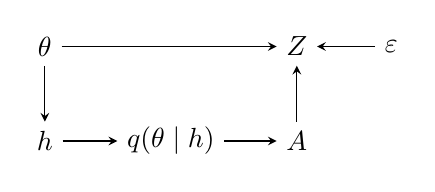
\begin{tikzpicture}[>=stealth, baseline=(th.base)]
\node (th) at (0,0) {$\theta$};
\node (h) at (0,-1.2) {$h$};
\node (q) at (1.6,-1.2) {$q(\theta\mid h)$};
\node (A) at (3.2,-1.2) {$A$};
\node (Z) at (3.2,0) {$Z$};
\node (e) at (4.4,0) {$\varepsilon$};
\draw[->] (th) -- (Z);
\draw[->] (th) -- (h);
\draw[->] (h) -- (q);
\draw[->] (q) -- (A);
\draw[->] (A) -- (Z);
\draw[->] (e) -- (Z);
\end{tikzpicture}
\end{center}
the difference is that $S$ has split: the outcome depends on $\theta$, the action on $q$, and the only link between them runs through past outcomes in $h$.
This posterior is over the channel, the model of (2b), and not a belief over a hidden state; the state here is trivial.

\paragraph{The gooder regulator.}
The graph above is Wentworth's Step~1, which only says the regulator acts on a function of $q$; to see when it must carry $q$ itself we need his Step~2.
We write $A$ for his regulator output $R$, since it is our action.
The regulator sees $X$, compresses it into a memory $M$, and only then receives $Y$, before acting with $A=f(M,Y)$.
His objective is
\begin{equation}
  \max_{f}\ \sum u(Z)\,P(Z\mid A,S,Y)\,P(A\mid M,Y)\,P(S\mid X)\,P(X)\,P(Y),
  \label{eq:gooder}
\end{equation}
so $Y$ is drawn independently of $S$ and $X$ and enters the kernel of the outcome: $Y$ chooses which game is played.
In our formalism $Y$ sits where $\varepsilon$ sits, an input to the kernel of $Z$ independent of the system, with one difference: $Y$ is seen after $M$ is fixed and before $A$ is chosen, so $A$ can depend on it, while $\varepsilon$ is realised after $A$ and never seen.
In the terms of \nolinkurl{good-regulator-information-theoretic.tex}, $Y$ is the part of the disturbance under cause control, $\varepsilon$ the part no regulator can counter, and $\theta$ the part reached only through the outcomes it has shaped, under error control.
If $M$ is minimal and for any two different posteriors $P(S\mid X)$ some $Y$ makes the optimal actions differ, then $M$ is the posterior up to relabelling.
In our terms $Y$ selects the channel, for instance which set of outcomes counts as desirable, so the bandit version has $Z\sim K_Y(\cdot\mid\theta,a)$,
\begin{center}
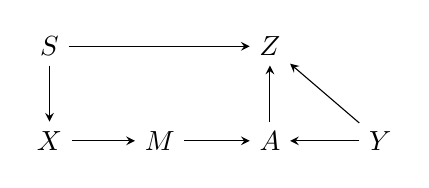
\begin{tikzpicture}[>=stealth, baseline=(S.base)]
\node (S) at (0,0) {$S$};
\node (X) at (0,-1.2) {$X$};
\node (M) at (1.4,-1.2) {$M$};
\node (A) at (2.8,-1.2) {$A$};
\node (Y) at (4.2,-1.2) {$Y$};
\node (Z) at (2.8,0) {$Z$};
\draw[->] (S) -- (X);
\draw[->] (X) -- (M);
\draw[->] (M) -- (A);
\draw[->] (Y) -- (A);
\draw[->] (S) -- (Z);
\draw[->] (A) -- (Z);
\draw[->] (Y) -- (Z);
\end{tikzpicture}
\hspace{16mm}
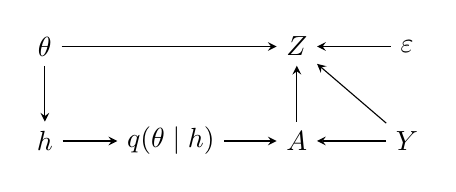
\begin{tikzpicture}[>=stealth, baseline=(th.base)]
\node (th) at (0,0) {$\theta$};
\node (h) at (0,-1.2) {$h$};
\node (q) at (1.6,-1.2) {$q(\theta\mid h)$};
\node (A) at (3.2,-1.2) {$A$};
\node (Y) at (4.6,-1.2) {$Y$};
\node (Z) at (3.2,0) {$Z$};
\node (e) at (4.6,0) {$\varepsilon$};
\draw[->] (th) -- (Z);
\draw[->] (th) -- (h);
\draw[->] (h) -- (q);
\draw[->] (q) -- (A);
\draw[->] (Y) -- (A);
\draw[->] (A) -- (Z);
\draw[->] (Y) -- (Z);
\draw[->] (e) -- (Z);
\end{tikzpicture}
\end{center}
With a single channel, as in~\eqref{eq:bandit-obj}, $Y$ takes one value and Step~2 does not apply.
It would apply if the desirable set were chosen after $h$ is seen: an arm's parameter for each choice is the probability of landing in that set, so a memory good for every choice must keep the posterior over the arm's whole outcome distribution, not over one hit rate.
This is the rich family that the gooder-regulator reading of (2b) found met only loosely.

With one fixed channel, a single round needs less than $q$: the predictive regulator needs only the means $\hat\theta_a$, the expected one only the values~\eqref{eq:arm-value} below.
What forces the counts over the mean is the repetition, a reason separate from Step~2.
Take $N=4$, so $F$ is decreasing above $1/(N+1)$, a known arm at $\theta=0.45$, and a second arm under either $\mathrm{Beta}(1,1)$ or $\mathrm{Beta}(10,10)$.
Both posteriors have mean $\tfrac12$, so the predictive regulator pulls the second arm under both.
After one miss the means are $\tfrac13$ and $\tfrac{10}{21}\approx0.48$, so it switches to the known arm under the first and stays under the second.
A memory holding only the mean cannot tell the two histories apart, and for Beta posteriors a memory that can is the counts, that is $q$.
The future data are not Wentworth's $Y$, since they depend on $\theta$; they are more of $X$, and the posterior is what the regulator must carry to update on them.

The same slots hold the other branches of the plan, which is how (2b) and (2c) stay distinct:
\begin{center}
\begin{tabular}{lllll}
\toprule
setting & $S$, what $Z$ depends on & $X$, what is seen & $M$, what is carried & disturbance \\
\midrule
bandit & $\theta$ & $h$ & $q(\theta\mid h)$ & $\varepsilon$ in $K$ \\
DeepSea, (2b) & $(s,\theta)$ & $(s,h)$ & $\big(s,q(\theta\mid h)\big)$ & $\varepsilon$ in $K$ \\
noisy sensor, (2c) & $s$ & $o_{1:t}$ & $b_t(s)$ & in $P$ or $K$ \\
\bottomrule
\end{tabular}
\end{center}
$S$ is everything the outcome depends on that the regulator does not choose, other than the game $Y$, and $M$ is the posterior over the part of it that is not seen: the channel parameter in (2b), the state in (2c).
The disturbance is not a node of Wentworth's graph but sits in the kernels.
In $P$ it is Conant and Ashby's arrow $D\to S$, the state being moved; in $K$ it is $\varepsilon\to Z$, the outcome being redrawn, and the bandit has only the second.

\paragraph{Two objectives, one simplex.}
With $\theta$ unknown there are two ways to put $q$ into~\eqref{eq:bandit-obj}, the predictive and the expected objectives of Section~\ref{sec:model}.
With $\hat\theta_a=\E_q[\theta_a]$ and $\hat R(\pi)=\sum_a\pi(a)\hat\theta_a$,
\begin{equation}
  J_{\mathrm{pred}}(\pi)=F\big(\hat R(\pi)\big),
  \qquad
  J_{\mathrm{exp}}(\pi)=\E_q\Big[F\big(R_\theta(\pi)\big)\Big]
  =J_{\mathrm{pred}}(\pi)-I_\pi(\theta;Z),
  \label{eq:bandit-two}
\end{equation}
the second equality being~\eqref{eq:expected-vs-predictive} with $I_\pi(\theta;Z)=h_b(\hat R)-\E_q h_b(R_\theta)$ from~\eqref{eq:info-gain}.
Both are concave on the simplex, $J_{\mathrm{exp}}$ as an average of concave functions, so both are minimised at an arm.
The regulator commits under either; what differs is which arm.
This is the static view, against a fixed $q$; Section~\ref{sec:belief} lets $q$ move and keeps only $J_{\mathrm{pred}}$.

\paragraph{The value of an arm.}
Since the minimiser is an arm, we only need the objectives at the vertices.
At $\pi=\delta_a$ the return is $\theta_a$, and the information term is the information one outcome of arm $a$ carries about its parameter,
\begin{equation}
  J_{\mathrm{pred}}(\delta_a)=F(\hat\theta_a),
  \qquad
  J_{\mathrm{exp}}(\delta_a)=F(\hat\theta_a)-I_a,
  \qquad
  I_a=I(\theta;Z\mid A=a)=h_b(\hat\theta_a)-\E_q\big[h_b(\theta_a)\big],
  \label{eq:arm-value}
\end{equation}
since with all mass on one arm there is no pair to forget, and the inequality $I(\theta;Z)\le I(\theta;Z\mid S,A)$ of Section~\ref{sec:model} holds with equality.
The predictive regulator picks the arm with the best mean; the expected regulator discounts each arm by what it would learn there.
For an unpulled arm under $\mathrm{Beta}(1,1)$, $\hat\theta_a=\tfrac12$ and
\begin{equation}
  I_a=\ln2-\int_0^1h_b(u)\,\dd u=\ln2-\tfrac12\approx0.19\ \text{nats},
\end{equation}
so against a known arm with $\theta=\tfrac12$ the two arms tie under $J_{\mathrm{pred}}$ and $J_{\mathrm{exp}}$ prefers the unpulled arm by $0.19$ nats.
A numerical check with $N=4$ and Beta posteriors $(1,1)$, $(3,2)$ and $(1,3)$ reproduces $J_{\mathrm{exp}}(\delta_a)=F(\hat\theta_a)-I_a$ to six decimals.

\paragraph{Where empowerment sits.}
To see which budget term the choice uses, we write~\eqref{eq:budget} for one state, where the localisation term vanishes, $\Hf{Z}=I(A;Z)+\Hf{Z\mid A}$.
For each $\theta$ this gives
\begin{equation}
  J_{\mathrm{exp}}(\pi)=\E_q\Big[I_\theta(A;Z)+\Hf{Z\mid A,\theta}\Big],
\end{equation}
and at every vertex $I_\theta(A;Z)=0$, since $A$ is constant.
So the value~\eqref{eq:arm-value} of every arm is the expected noise term $\E_q\big[F(\theta_a)\big]$ alone, and empowerment does not enter the choice.
Klyubin's capacity $C_\theta=\max_pI_p(A;Z\mid\theta)$ is still positive whenever the $\theta_a$ differ: the regulator has leverage over $Z$, and it spends it by choosing an arm, not by randomising over them.
On the predictive channel the capacity is zero while the $\hat\theta_a$ are equal, as they are before any pull.
What separates the arms before any pull is $I_a$, information about the channel at the arm the regulator commits to.

\paragraph{The loop, and what it leaves open.}
Each round the regulator pulls the arm minimising~\eqref{eq:arm-value}, updates $q$, and recomputes.
The (2b) Thompson variant instead draws $\theta\sim q$ and pulls the minimiser of $F(\theta_a)$, which under the threshold is the arm of largest sampled $\theta_a$, Thompson sampling for a Bernoulli bandit.
Neither values what a pull will teach for later rounds: the objective is static in the sense of Section~\ref{sec:model}, and $I_a$ enters only through the concavity of $F$ at the current round.
And the occupancy is a long-run frequency, while $q$ changes as the data are collected, so the objective the loop descends at round $k$ is not the entropy of the outcomes the regulator actually sees over its rounds; that is the single-lifetime caveat of (2c), logged in the plan and not pursued here.

\section{The Belief as State: Occupancy over Beliefs}
\label{sec:belief}
Added 24 September 2026.
Section~\ref{sec:bandit} chose one arm against a fixed posterior, so nothing in it accounts for how the posterior contracts as data arrive.
Here we apply the objective~\eqref{eq:obj} as it stands to the MDP whose state is the posterior, so that the contraction enters through the occupancy.
We ask what the objective becomes, when it degenerates, and what disturbance makes it meaningful.

\paragraph{The belief MDP.}
We need one new object, the MDP over posteriors, because the occupancy has to be taken over the states the regulator actually acts on.
Its state is the posterior $b=q(\theta\mid h)$, Beta counts per arm in the bandit, and its two kernels are the predictive ones,
\begin{equation}
  \bar K(z\mid b,a)=\E_{\theta\sim b}\big[K_{\theta_a}(z)\big]=K_{\hat\theta_a(b)}(z),
  \qquad
  P(b'\mid b,a)=\sum_z\bar K(z\mid b,a)\,\1\big\{b'=u(b,a,z)\big\},
  \label{eq:belief-mdp}
\end{equation}
with $\hat\theta_a(b)=\E_b[\theta_a]$, $u$ the Bayes update, and the first equality~\eqref{eq:channel-affine} applied to the posterior.
Starting from $b_0=q_0$, a stationary belief policy $\pi(a\mid b)$ has an occupancy $\occ(b,a)$ that satisfies the flow constraint of v1 with this $P$.
The feasible set is again a polytope, its vertices are deterministic belief policies, and the objective is~\eqref{eq:obj} with $\bar K$ as the channel, $\min_\pi\Hf{\occ\bar K}$.
Pulling an uncertain arm moves the occupancy towards sharper beliefs, and that is the only route by which the contraction reaches $Z$.

\paragraph{The objective factors through the Bayesian return.}
Every $\bar K(\cdot\mid b,a)$ is a member of the family~\eqref{eq:K-family}, so the factorisation of v1 applies without change.
Averaging~\eqref{eq:belief-mdp} over the occupancy with~\eqref{eq:channel-affine},
\begin{equation}
  \occ\bar K=K_{\hat R(\pi)},
  \qquad
  \hat R(\pi)=\sum_{b,a}\occ(b,a)\,\hat\theta_a(b),
  \qquad
  \Hf{\occ\bar K}=F\big(\hat R(\pi)\big),
  \label{eq:belief-factor}
\end{equation}
where $\hat R$ is the Bayesian return, the return of the belief MDP with reward $\hat\theta_a(b)$.
Under~\eqref{eq:stoch-channel-condition} the homeostasis optimum is therefore the Bayes-optimal policy, which values what a pull will teach.
This is the predictive objective of Section~\ref{sec:model}, and there it explored only through an optimistic prior mean because it scored one policy against a fixed $q$; on the belief MDP the same objective is Bayes-adaptive.

\paragraph{The predictive outcome law is the true one.}
We use only~\eqref{eq:belief-factor}, and one identity shows it needs no companion objective: the law it scores is the law of the outcomes the regulator actually produces.
Since $b_t=q(\theta\mid h_t)$ and $b_t$ is a function of $h_t$, conditioning on $b_t$ averages the posterior over the histories that produce it,
\begin{equation}
  P(\theta\mid b_t=b)=\E\big[q(\theta\mid h_t)\,\big|\,b_t=b\big]=b(\theta),
\end{equation}
so for every $t$, $P(\theta,b_t=b,a_t=a)=P(b_t=b)\,\pi(a\mid b)\,b(\theta)$, and summing over $t$ with the discount weights,
\begin{equation}
  d(\theta,b,a)=\occ(b,a)\,b(\theta).
  \label{eq:joint-occ}
\end{equation}
The outcome law of the run, with $\theta$ drawn by the world and $Z$ by the true channel, is then
\begin{equation}
  p(z)=\sum_{\theta,b,a}d(\theta,b,a)\,K_{\theta_a}(z)
  =\sum_{b,a}\occ(b,a)\sum_\theta b(\theta)\,K_{\theta_a}(z)
  =(\occ\bar K)(z),
\end{equation}
by~\eqref{eq:joint-occ} and then~\eqref{eq:belief-mdp}.
So $\min_\pi\Hf{\occ\bar K}$ is Conant and Ashby's criterion taken over everything the regulator does not control, $\theta$ included, with no approximation.
Conditioning on $\theta$ as well gives the expected objective of Section~\ref{sec:model}, which was introduced to put an information term into an objective that could not see learning; here the occupancy carries the learning, and we drop it.
The objective is concave in $\occ$, so a deterministic belief policy is optimal, which is the gooder-regulator conclusion with the belief as state.

\paragraph{Resets, observed and hidden.}
We now check the two occupancies of v2 against this MDP, and find that both are one construction.
With $\theta$ drawn once, the counts only grow, no belief is visited twice, and the belief chain is not unichain.
In the average occupancy the steps spent learning then have weight zero, every policy that eventually identifies the best arm has the same $\hat R$, and the objective does not price learning; this is the condition of v1 read at the level of the belief, the objective has meaning only under a persistent disturbance.
The discounted occupancy supplies one, by the reading of $\gamma$ in v1 as a termination probability: at each step, with probability $1-\gamma$, the episode restarts, $\theta$ is redrawn from $q_0$ and the belief returns to $q_0$.
The same process for $\theta$, written with a rate $\eta$,
\begin{equation}
  \theta_{t+1}=\theta_t\ \text{with probability }1-\eta,
  \qquad
  \theta_{t+1}\sim q_0\ \text{with probability }\eta,
  \label{eq:drift}
\end{equation}
is Conant and Ashby's arrow $D\to S$ with $S=\theta$, and it admits two regulators.
If the redraw is observed, as the restart indicator $d_t$ is in v1, the belief jumps to $q_0$ and this is the discounted occupancy with $1-\gamma=\eta$.
If it is hidden, the posterior over $\theta_{t+1}$ given $h_{t+1}$ is the update followed by the same mixture,
\begin{equation}
  b_{t+1}=(1-\eta)\,u(b_t,a_t,z_t)+\eta\,q_0 ,
  \label{eq:belief-relax}
\end{equation}
so observation contracts the belief at the arm pulled, and the disturbance relaxes it towards the prior at every arm.
In both cases the belief chain returns to a stationary regime, the average occupancy is not degenerate, and $b_t$ is the posterior over the current $\theta_t$, so~\eqref{eq:joint-occ} holds and the outcome law of the run is still $\occ\bar K$.
The difference is only whether the regulator sees the disturbance: an observed reset is under cause control, like $Y$, and a hidden one reaches the regulator only through outcomes, like $\theta$ itself.
In the slot table of Section~\ref{sec:bandit} the bandit now has both disturbances, $\varepsilon$ in $K$ and~\eqref{eq:drift} in $P$.

\paragraph{Where $\min_\pi\Hf{Z}$ pays for not knowing.}
The objective is unchanged, so we only need to see how~\eqref{eq:belief-relax} moves the predictive channel.
An arm left unpulled for $k$ steps has $b\to(1-\eta)^k b+\big(1-(1-\eta)^k\big)q_0$, so $\hat\theta_a\to\E_{q_0}[\theta_a]$ and its predicted outcome relaxes to $K_{\E_{q_0}\theta_a}$.
For an arm the regulator has learned to be good, that is a more uniform outcome, and $F$ charges it at every step of the long-run average.
So not knowing is paid for as outcome entropy, the homeostasis way, and the regulator must keep pulling to hold its belief sharp against the drift.
Two limits of this accounting.
$\bar K$ sees $b$ only through its mean, so a wide belief with a good mean costs nothing by itself; what is charged is the outcome the regulator can expect.
And one pull carries at most $\ln2$ nats about $\theta$, by the argument of~\eqref{eq:emp-binary-general}, which suggests that tracking is possible only while $\eta$ is small against that rate; this is a conjecture, not derived here.

\paragraph{A numerical check.}
We solve a restless two-arm bandit to see whether the optimum tracks.
Arm $0$ is known with $\theta_0=0.55$; arm $1$ has $\theta_1\in\{0.2,0.8\}$ under $q_0=(\tfrac12,\tfrac12)$ with the drift~\eqref{eq:drift}, so the belief is the scalar $p=P(\theta_1=0.8)$, and $N=4$.
Every parameter is at least $0.2=1/(N+1)$, so every policy has $\hat R\ge1/(N+1)$, where $F$ is decreasing, so by~\eqref{eq:belief-factor} minimising $F(\hat R)$ is maximising $\hat R$.
We solve that by value iteration on a grid of $p$ with $\gamma=0.999$ as a stand-in for the average, and simulate $4\cdot10^5$ steps.
With the redraw hidden, the optimum pulls arm $1$ exactly when $p$ exceeds a threshold $p^\ast$; the stay is the mean number of steps on arm $0$ before returning.
The last two columns solve the same problem with the redraw observed.
\begin{center}
\begin{tabular}{lcccccc}
\toprule
& \multicolumn{4}{c}{hidden redraw~\eqref{eq:belief-relax}} & \multicolumn{2}{c}{observed redraw} \\
\cmidrule(lr){2-5}\cmidrule(lr){6-7}
$\eta$ & $p^\ast$ & stay on arm $0$ & $\hat R$ & $F(\hat R)$ & $\hat R$ & $F(\hat R)$ \\
\midrule
$0.001$ & $0.05$ & $75.6$ & $0.664$ & $1.104$ & $0.672$ & $1.087$ \\
$0.01$ & $0.14$ & $22.7$ & $0.642$ & $1.148$ & $0.663$ & $1.106$ \\
$0.05$ & $0.27$ & $9.8$ & $0.618$ & $1.194$ & $0.643$ & $1.146$ \\
$0.2$ & $0.41$ & $4.7$ & $0.578$ & $1.266$ & $0.604$ & $1.220$ \\
\bottomrule
\end{tabular}
\end{center}
With the redraw observed the regulator never returns to arm $1$ between redraws: once it retires to the known arm it stays there until the next reset, where it starts learning again from the prior.
With the redraw hidden it has to keep checking, and the gap between the two $\hat R$ columns is the cost of not observing the disturbance.
For comparison, a regulator that knows $\theta_1$ reaches $\hat R=0.675$, and staying on the known arm gives $\hat R=0.55$, $F=1.312$.
The greedy regulator, which pulls arm $1$ only when its mean exceeds $0.55$, never does: at $p=\tfrac12$ the mean is $0.5$, and without pulls the belief stays at the prior.
The optimum returns sooner as the world moves faster, and the entropy it pays rises with $\eta$ towards that of the known arm.

\paragraph{What is open.}
The DeepSea analogue is a treasure that moves at rate $\eta$, on the belief state $(s,b)$, which is a Bayes-adaptive MDP and not tractable exactly.
Posterior sampling and the Thompson variant of (2b) then read as approximations to the optimum of~\eqref{eq:belief-factor}, not as objectives of their own, and v2's MM loop applies on the belief MDP as written.
The variety conjecture above is the check to run next.

\bibliographystyle{plainnat}
% Overleaf compiles from the project root, a local latexmk -cd from this folder; resolve the .bib paths either way.
\IfFileExists{notes_joery/joery.bib}
  {\newcommand{\bibs}{action-sufficient,notes_joery/joery}}
  {\newcommand{\bibs}{../action-sufficient,joery}}
\bibliography{\bibs}

\end{document}
